\subsection{Large scale simulations}
\label{sec:largescale}

To check validity of the small-scale experiment results, we performed a larger-scale evaluation based on a modified version of Rocketfuel AT\&T topology~\cite{rocketfuel}.
In order to approximate the general structure of the Internet,
% (scale-free structure, customer-provider, and peer-to-peer relations)
we extracted the largest connected component of 562 nodes from the original topology and separated nodes in three categories: clients, gateways, and backbones.
All nodes with degrees one, two, and three became clients (344 red nodes on Fig.~\ref{fig:large-scale}), all nodes that are directly connected to clients became gateways (109 green nodes), and the rest became backbones (109 blue nodes).
(To ensure that paths in the topology are ``valley-free,'' we augmented the topology with necessary backbone-to-backbone links.)
After categorizing the nodes, we randomly assigned bandwidths and link delays based on link types (see Table~\ref{tab:large-scale}).

\begin{figure}[htbp]
  \centering
  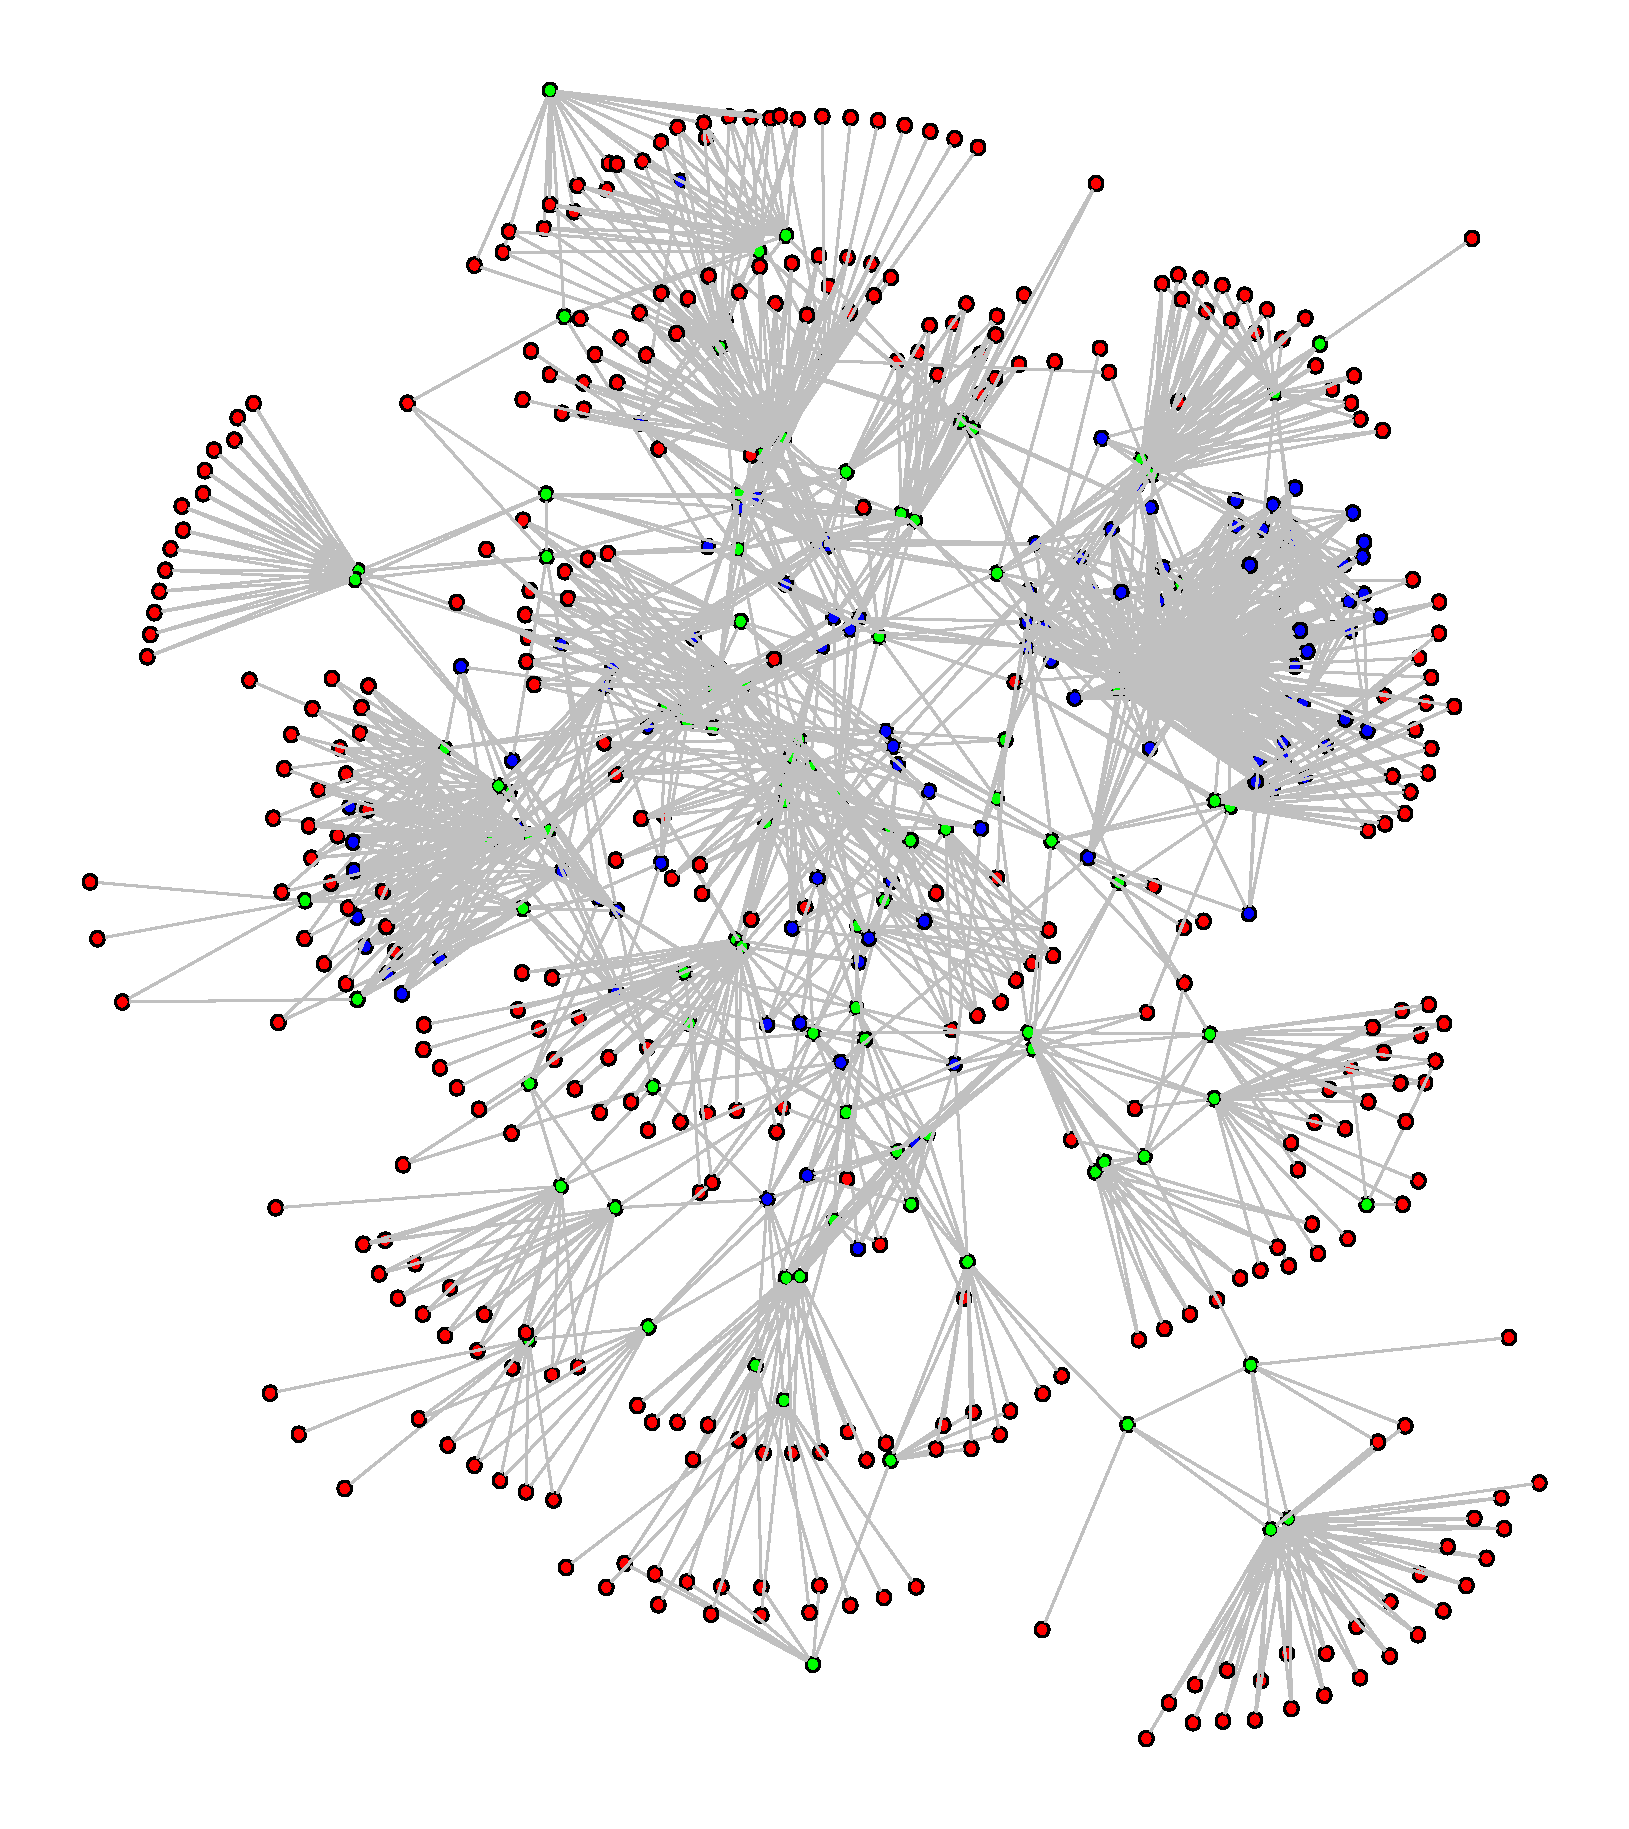
\includegraphics[scale=0.26,angle=90]{7018-r0}
  \caption{Internet-like topology: 344 client routers (red), 109 gateway routers (green), 109 backbone routers (blue)}
  \label{fig:large-scale-topo}
\end{figure}

\begin{table}[htbp]
\centering
\caption{Large-scale topology parameters}
\label{tab:large-scale}
\begin{tabular}{|l||c|c||c|c|}
  \hline
  \multirow{2}{*}{\bf Link type} &  \multicolumn{2}{|c||}{\bf Delay} &  \multicolumn{2}{|c|}{\bf Bandwidth} \tabularnewline
  \cline{2-5}
                        &  Min & Max                       &  Min & Max \tabularnewline
  \hline \hline
  Backbone--Backbone    & 5~ms & 10~ms   & 40~Mbps & 100~Mbps \tabularnewline
  \hline
  Gateway--Backbone,    & \multirow{2}{*}{5~ms} & \multirow{2}{*}{10~ms}   
                        & \multirow{2}{*}{10~Mbps} & \multirow{2}{*}{20~Mbps} \tabularnewline
  Gateway--Gateway      & & & & \\
  \hline
  Client--Gateway       & 10~ms & 70~ms   & 1~Mbps  & 3~Mbps \\
  \hline

\end{tabular}
\end{table}

In an Internet-like topology, the location of the Data producer plays the key part in his ability to sustain flooding attack.
That is, if the producer has limited network capacity (a personal blog located hosted on a client node), then he will be a really easy target for the attack.
On the other extreme, when the producer is located at the backbone (Google or Amamzon), then the attack would have a hard time to degrade service, as a lot of legitimate users would not even share paths with attackers.
To evaluate a balanced network scenario, we placed the Data producer at the gateway node, which randomly picked for each simulation run.
Similarly to the first set of small-scale evaluations, we fixed the number of malicious nodes at approximately 40\% level (140 out of 344 client nodes in the topology), while randomly varied which locations of compromised nodes.

% The results for all attack mitigation algorithms and all runs are aggregated in Fig.~\ref{fig:small-scale attack progress}, where Y-axis represents a minimum and maximum range for observed Interest satisfaction percentages among all nodes and all simulation runs.
% A short and simplistic summary of the results is that the first two attack mitigation methods do not work at all, and the last two are working quite good.

The evaluation results,\footnote{Note that for larger-scale experiments we reduced attack window to 15~minutes} summarized in Fig.~\ref{fig:large-scale}, show that for both physical limits algorithms and dynamic limits algorithm the performance is about the same as in small-scale evaluations (Fig.~\ref{fig:small-scale}), but with larger variations of minimum and maximum instantaneous satisfaction rates.

\begin{figure}[tbh]
 \centering
 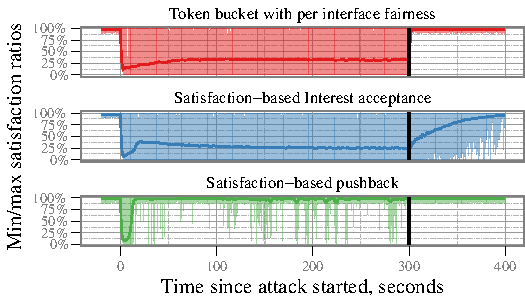
\includegraphics[scale=1]{topo-7018-gw-15mins-new/7018-r0-good-0-producer-gw}
 \caption{Satisfaction ratio dynamics during the attack (30\% attackers)}
 % producer on a gateway node
 \label{fig:large-scale}
\end{figure}

At the same time, the probabilistic method completely failed to provide an adequate protection against the Interest flooding attack, and in addition degraded service for the legitimate users after the attack finished.
The main reason for the failure was already explained in Section~\ref{sec:probabilistic}.
That is, if the number of hops between legitimate users and the Data producer is large (15 on average in the simulated topology) uncoordinated probabilistic Interest drops result in minuscule probability for good Interests to reach the Data producer during an ongoing attack, resulting in negative Interests satisfaction ratio statistics.
This also explains why until the statistics ages out, not all legitimate users can get satisfy all of their Interests.

In summary, in all of the simulated topologies, the dynamic limits algorithm restricts malicious traffic from even entering the network.
The only short periods of time when malicious Interests are getting admitted to the network is when routers have either no prior knowledge about per-interface satisfaction ratios (the initial period of the attack) or such knowledge becomes stale (statistics decaying during the attack).
As soon as the knowledge is obtained or refreshed, the service for legitimate users returns to norm.


% Alex: Anything else here?

% Alex: I also experimented with placing producer at the backbone, getting slightly better results for all algorithms.  Though I'm not sure there is any value to put those results in the paper


%%% Local Variables: 
%%% mode: latex
%%% TeX-master: "paper"
%%% End: 
